\section{Auswertung}

\subsection{Eichung des Elektromagneten}
\begin{table}
  \centering
  \caption{Messwerte der Magnetfeldstärke abhängig von der Stromstärke.}
  \label{tab:B}
  \begin{tabular}{S[table-format=2] S[table-format=3] S[table-format=3]}
    \toprule
    {$I$ / A} &  {$B$ / mT} & {$B$ / mT} \\
    {} & {(steigend)} & {(fallend)} \\
    \midrule
    0 &    4 &     5 \\
    1 &   71 &   74 \\
    2 &  129 &  131 \\
    3 &  195 &  179 \\
    4 &  253 &  240 \\
    5 &  307 &  308 \\
    6 &  368 &  370 \\
    7 &  428 &  420 \\
    9 &  556 &  555 \\
    8 &  488 &  472 \\
    10 & 614 &  609 \\
    11 & 661 &  668 \\
    12 & 723 &  730 \\
    13 & 777 &  779 \\
    14 & 830 &  841 \\
    15 & 872 &  888 \\
    16 & 948 &  923 \\
    17 & 972 &  972 \\
    \bottomrule
  \end{tabular}
\end{table}

lineare Regression der Form
\begin{equation}
  B(I) = aI + b
\end{equation}
ergibt
\begin{align*}
  a &= \SI{57.9 \pm 0.4}{\frac{mT}{A}} \\
  b &= \SI{18 \pm 4}{mT}
\end{align*}


\begin{figure}
  \centering
  \includegraphics{plots/plot.pdf}
  \caption{Plot.}
  \label{fig:plot}
\end{figure}

\subsection{Messung der Landé-Faktoren}

\begin{figure}
  \centering
  \begin{subfigure}{0.48\textwidth}
    \centering
    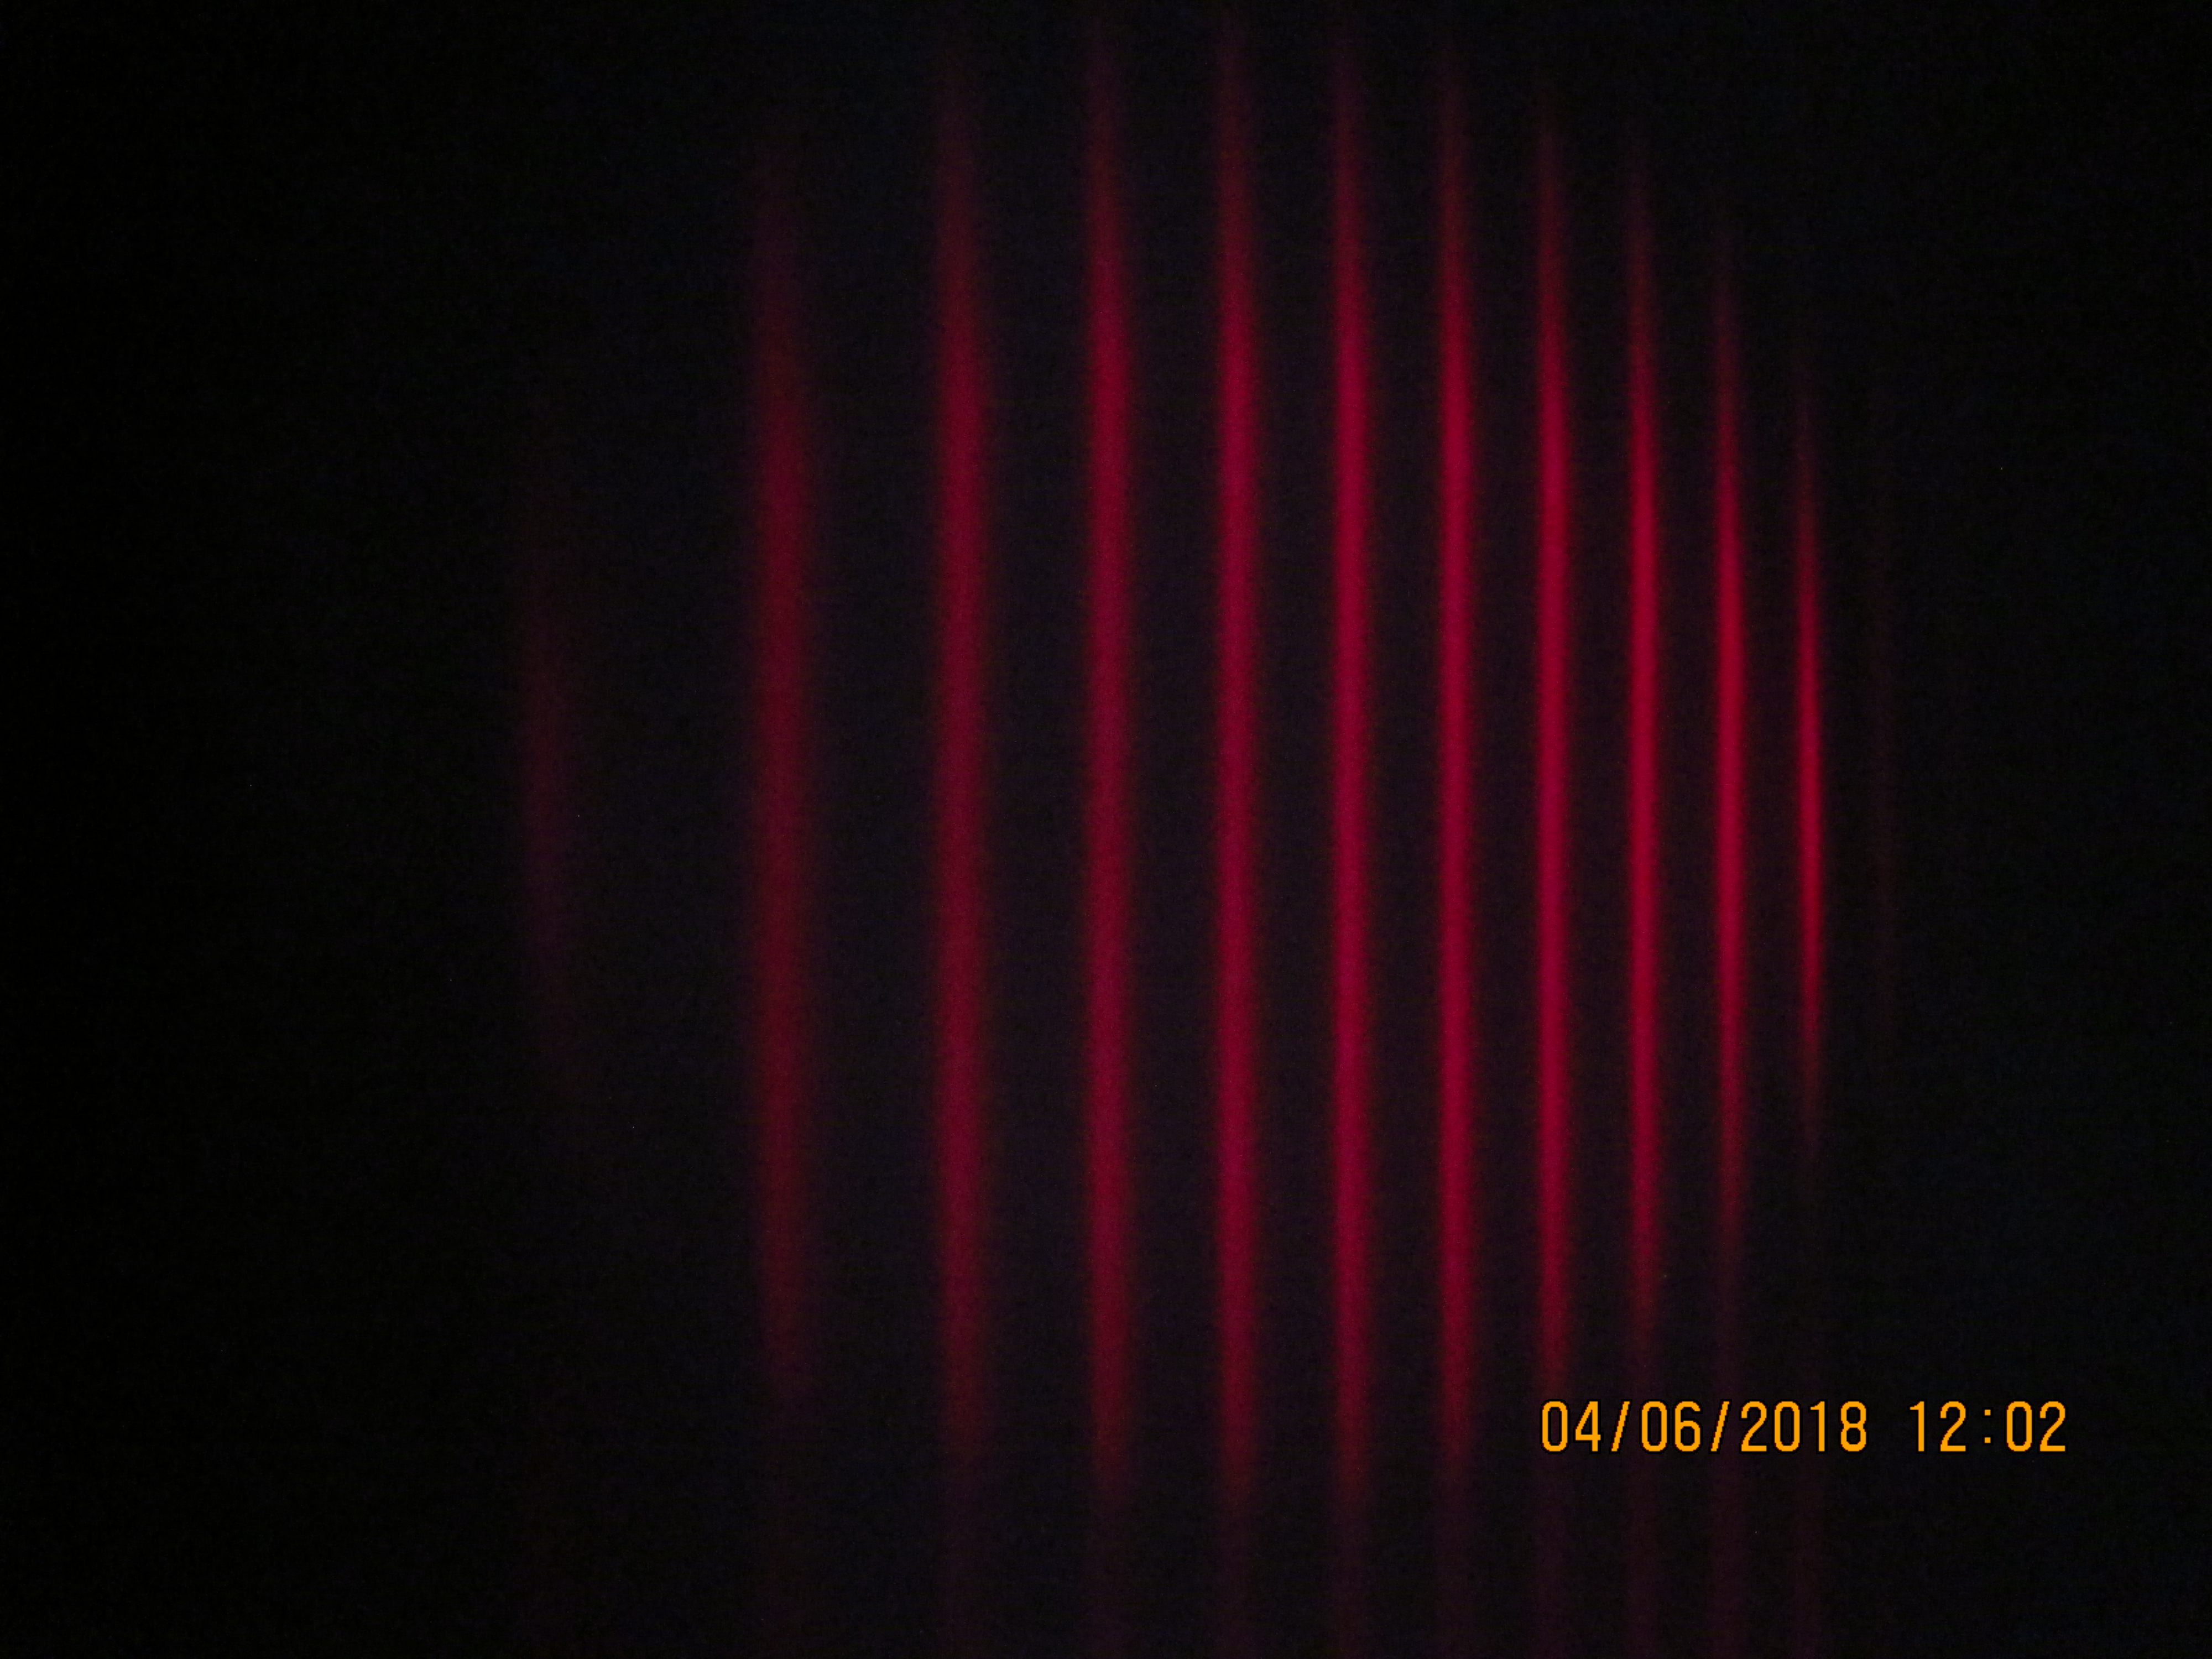
\includegraphics[width=\textwidth]{graphics/aufnahmen/IMG_1629.jpg}
    \caption{Aufnahme ohne Magnetfeld.}
  \end{subfigure}
  \begin{subfigure}{0.48\textwidth}
    \centering
    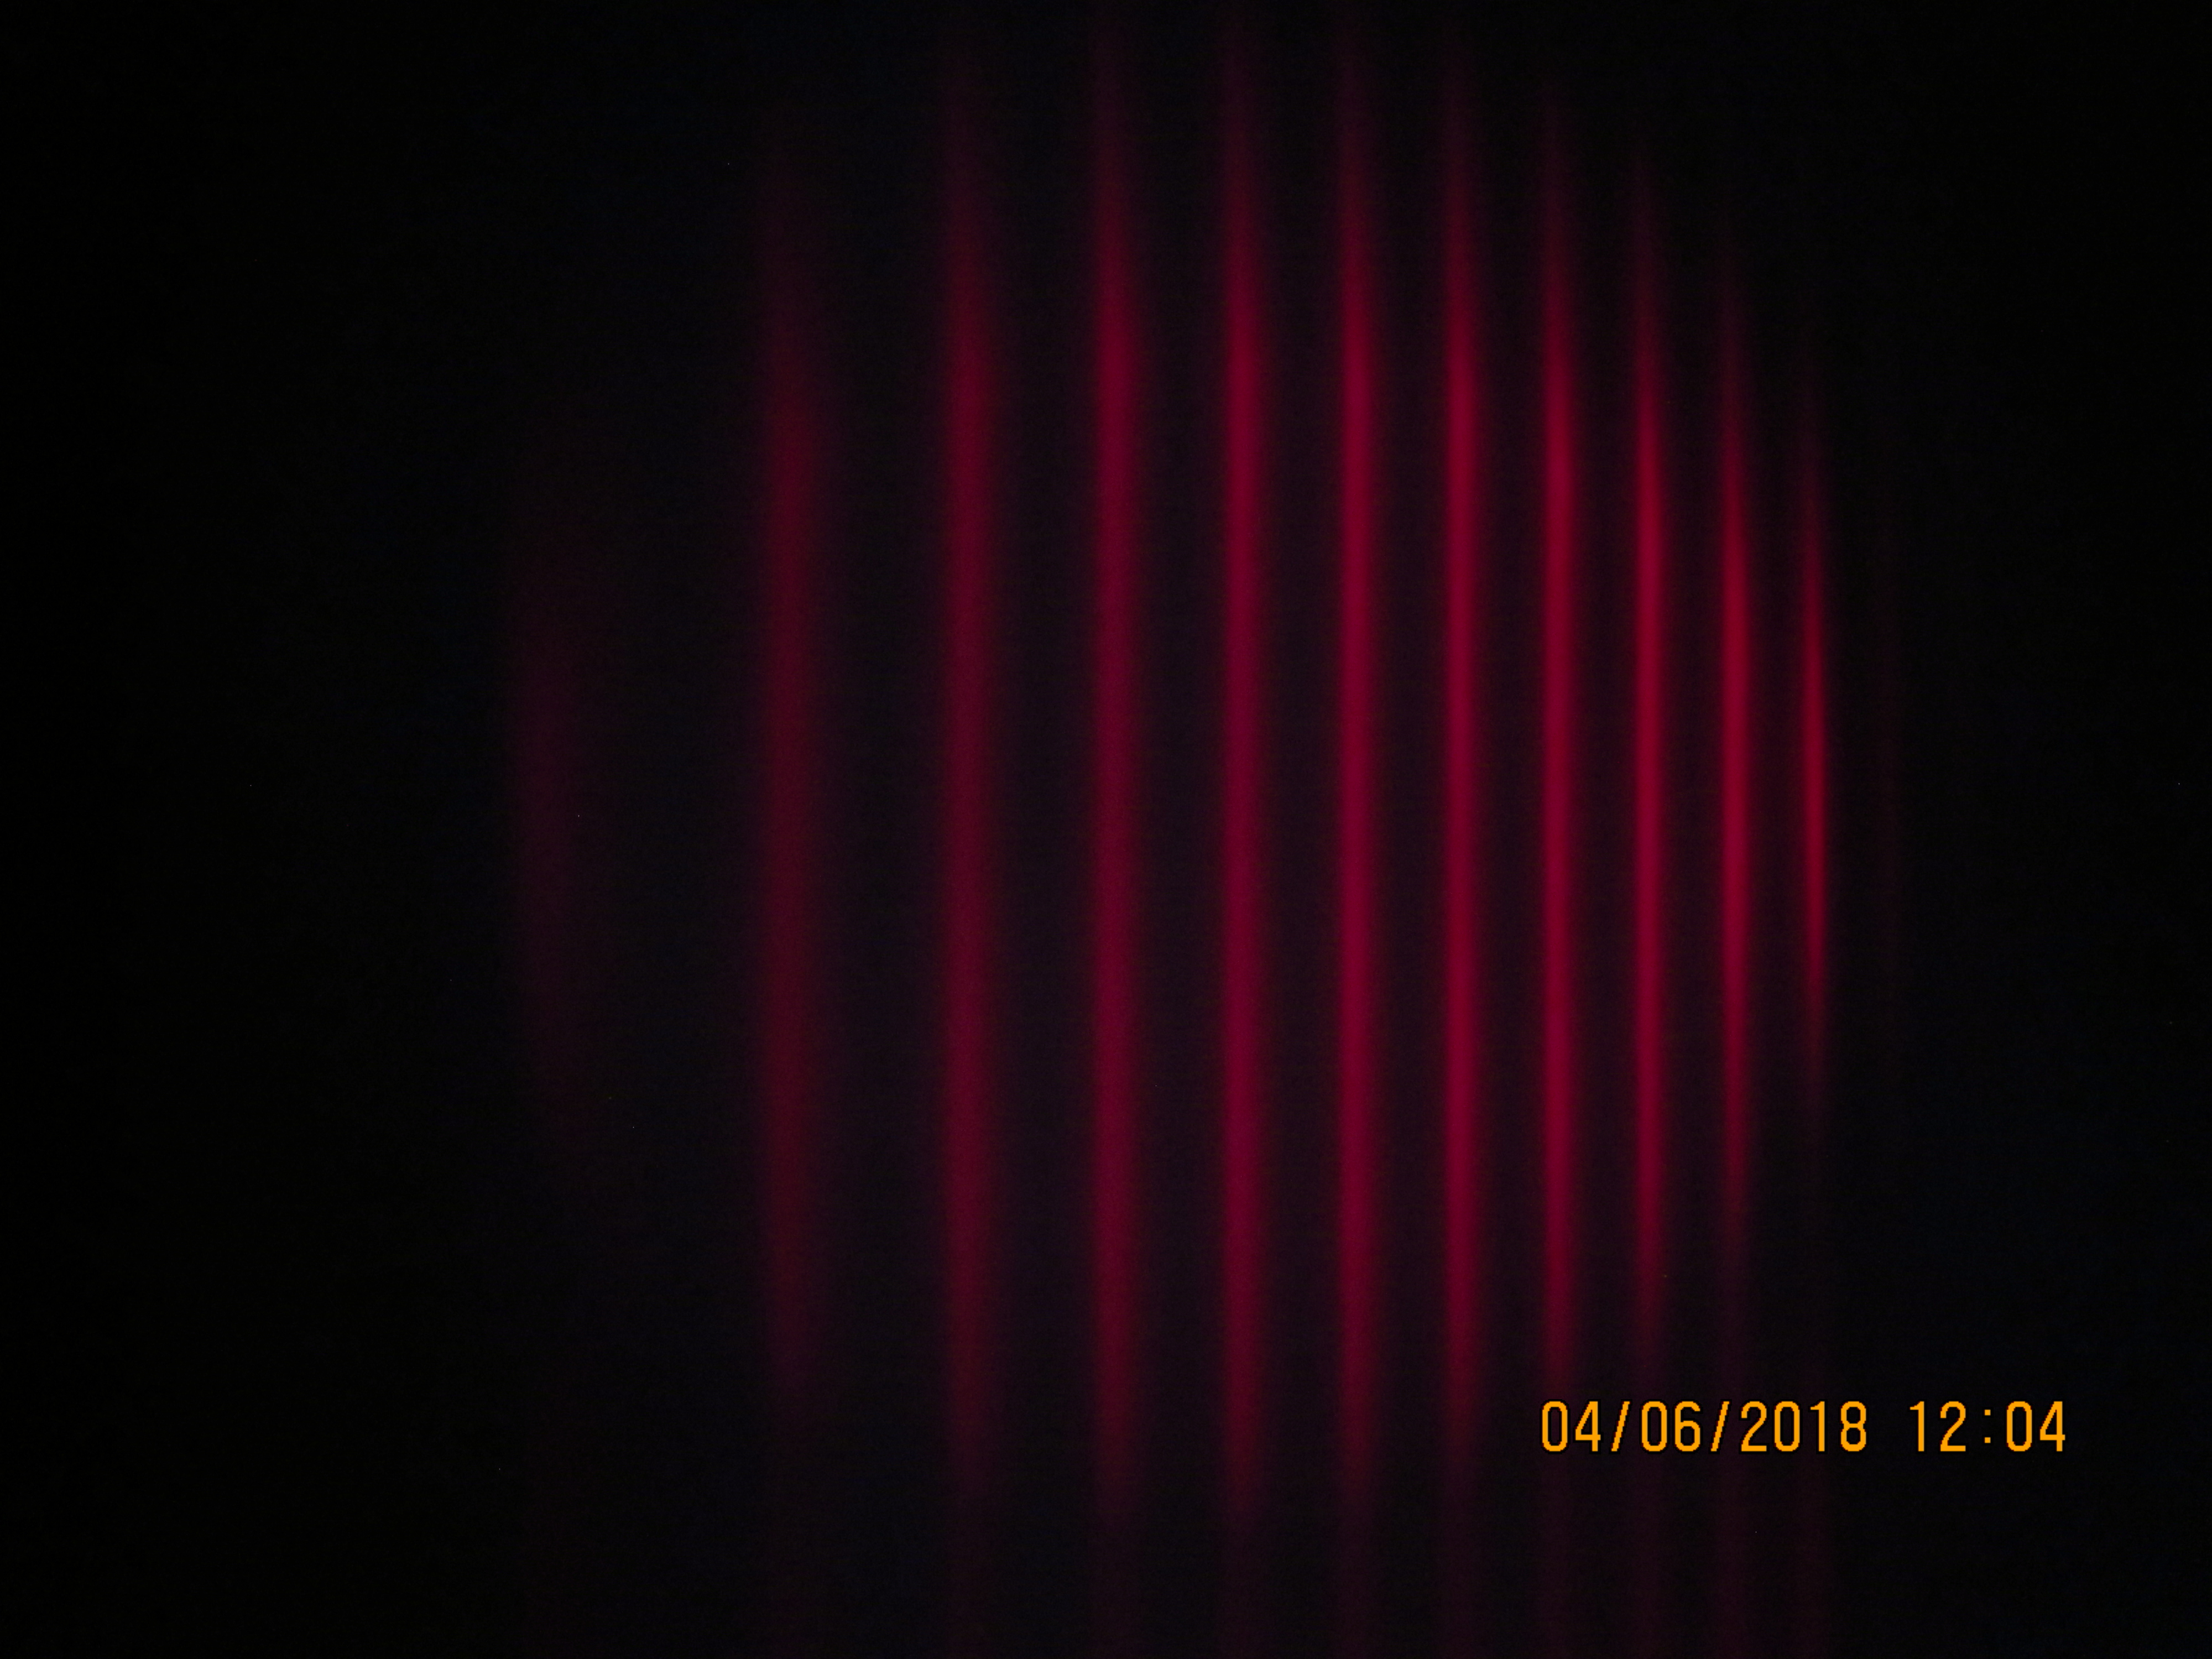
\includegraphics[width=\textwidth]{graphics/aufnahmen/IMG_1630.jpg}
    \caption{Aufnahme mit Magnetfeld.}
  \end{subfigure}
  \caption{rote $\pi$-Linie.}
  \label{fig:r_pi}
\end{figure}

\begin{figure}
  \centering
  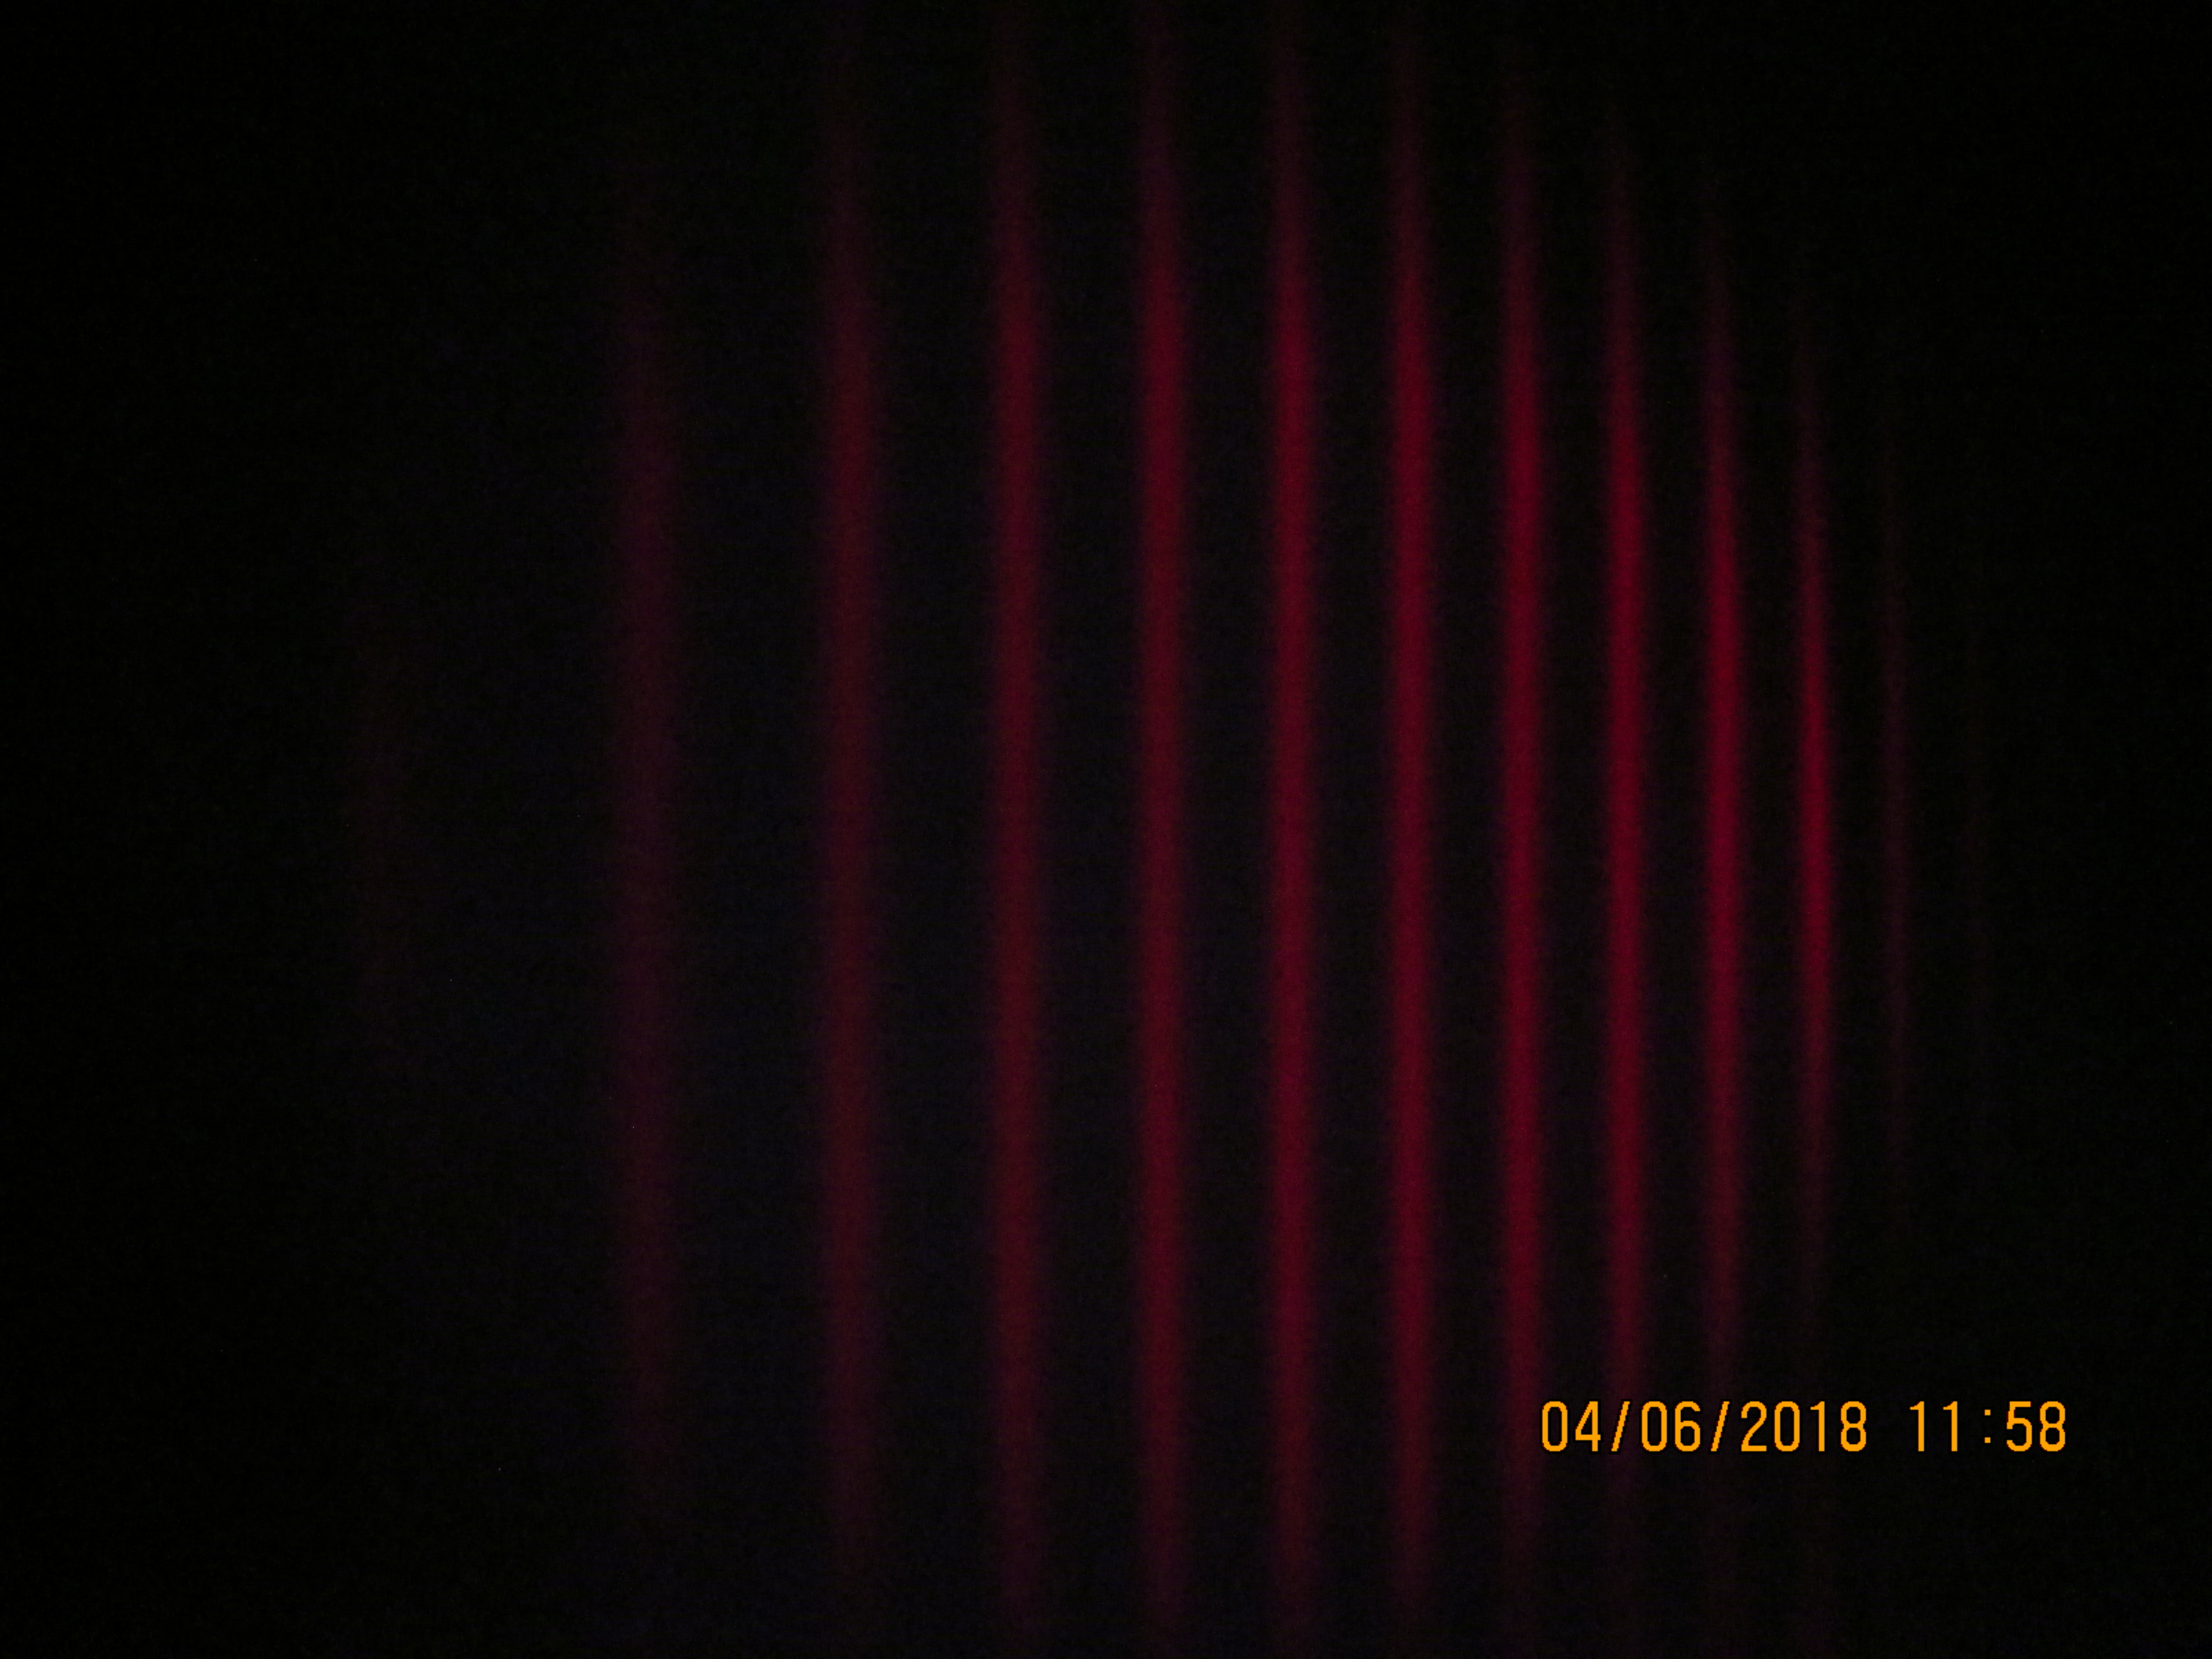
\includegraphics[width=0.95\textwidth]{graphics/auswertung/IMG_1627.png}
  \caption{rote $\sigma$-Linie ohne Magnetfeld.}
  \label{}
\end{figure}
\begin{figure}
  \centering
  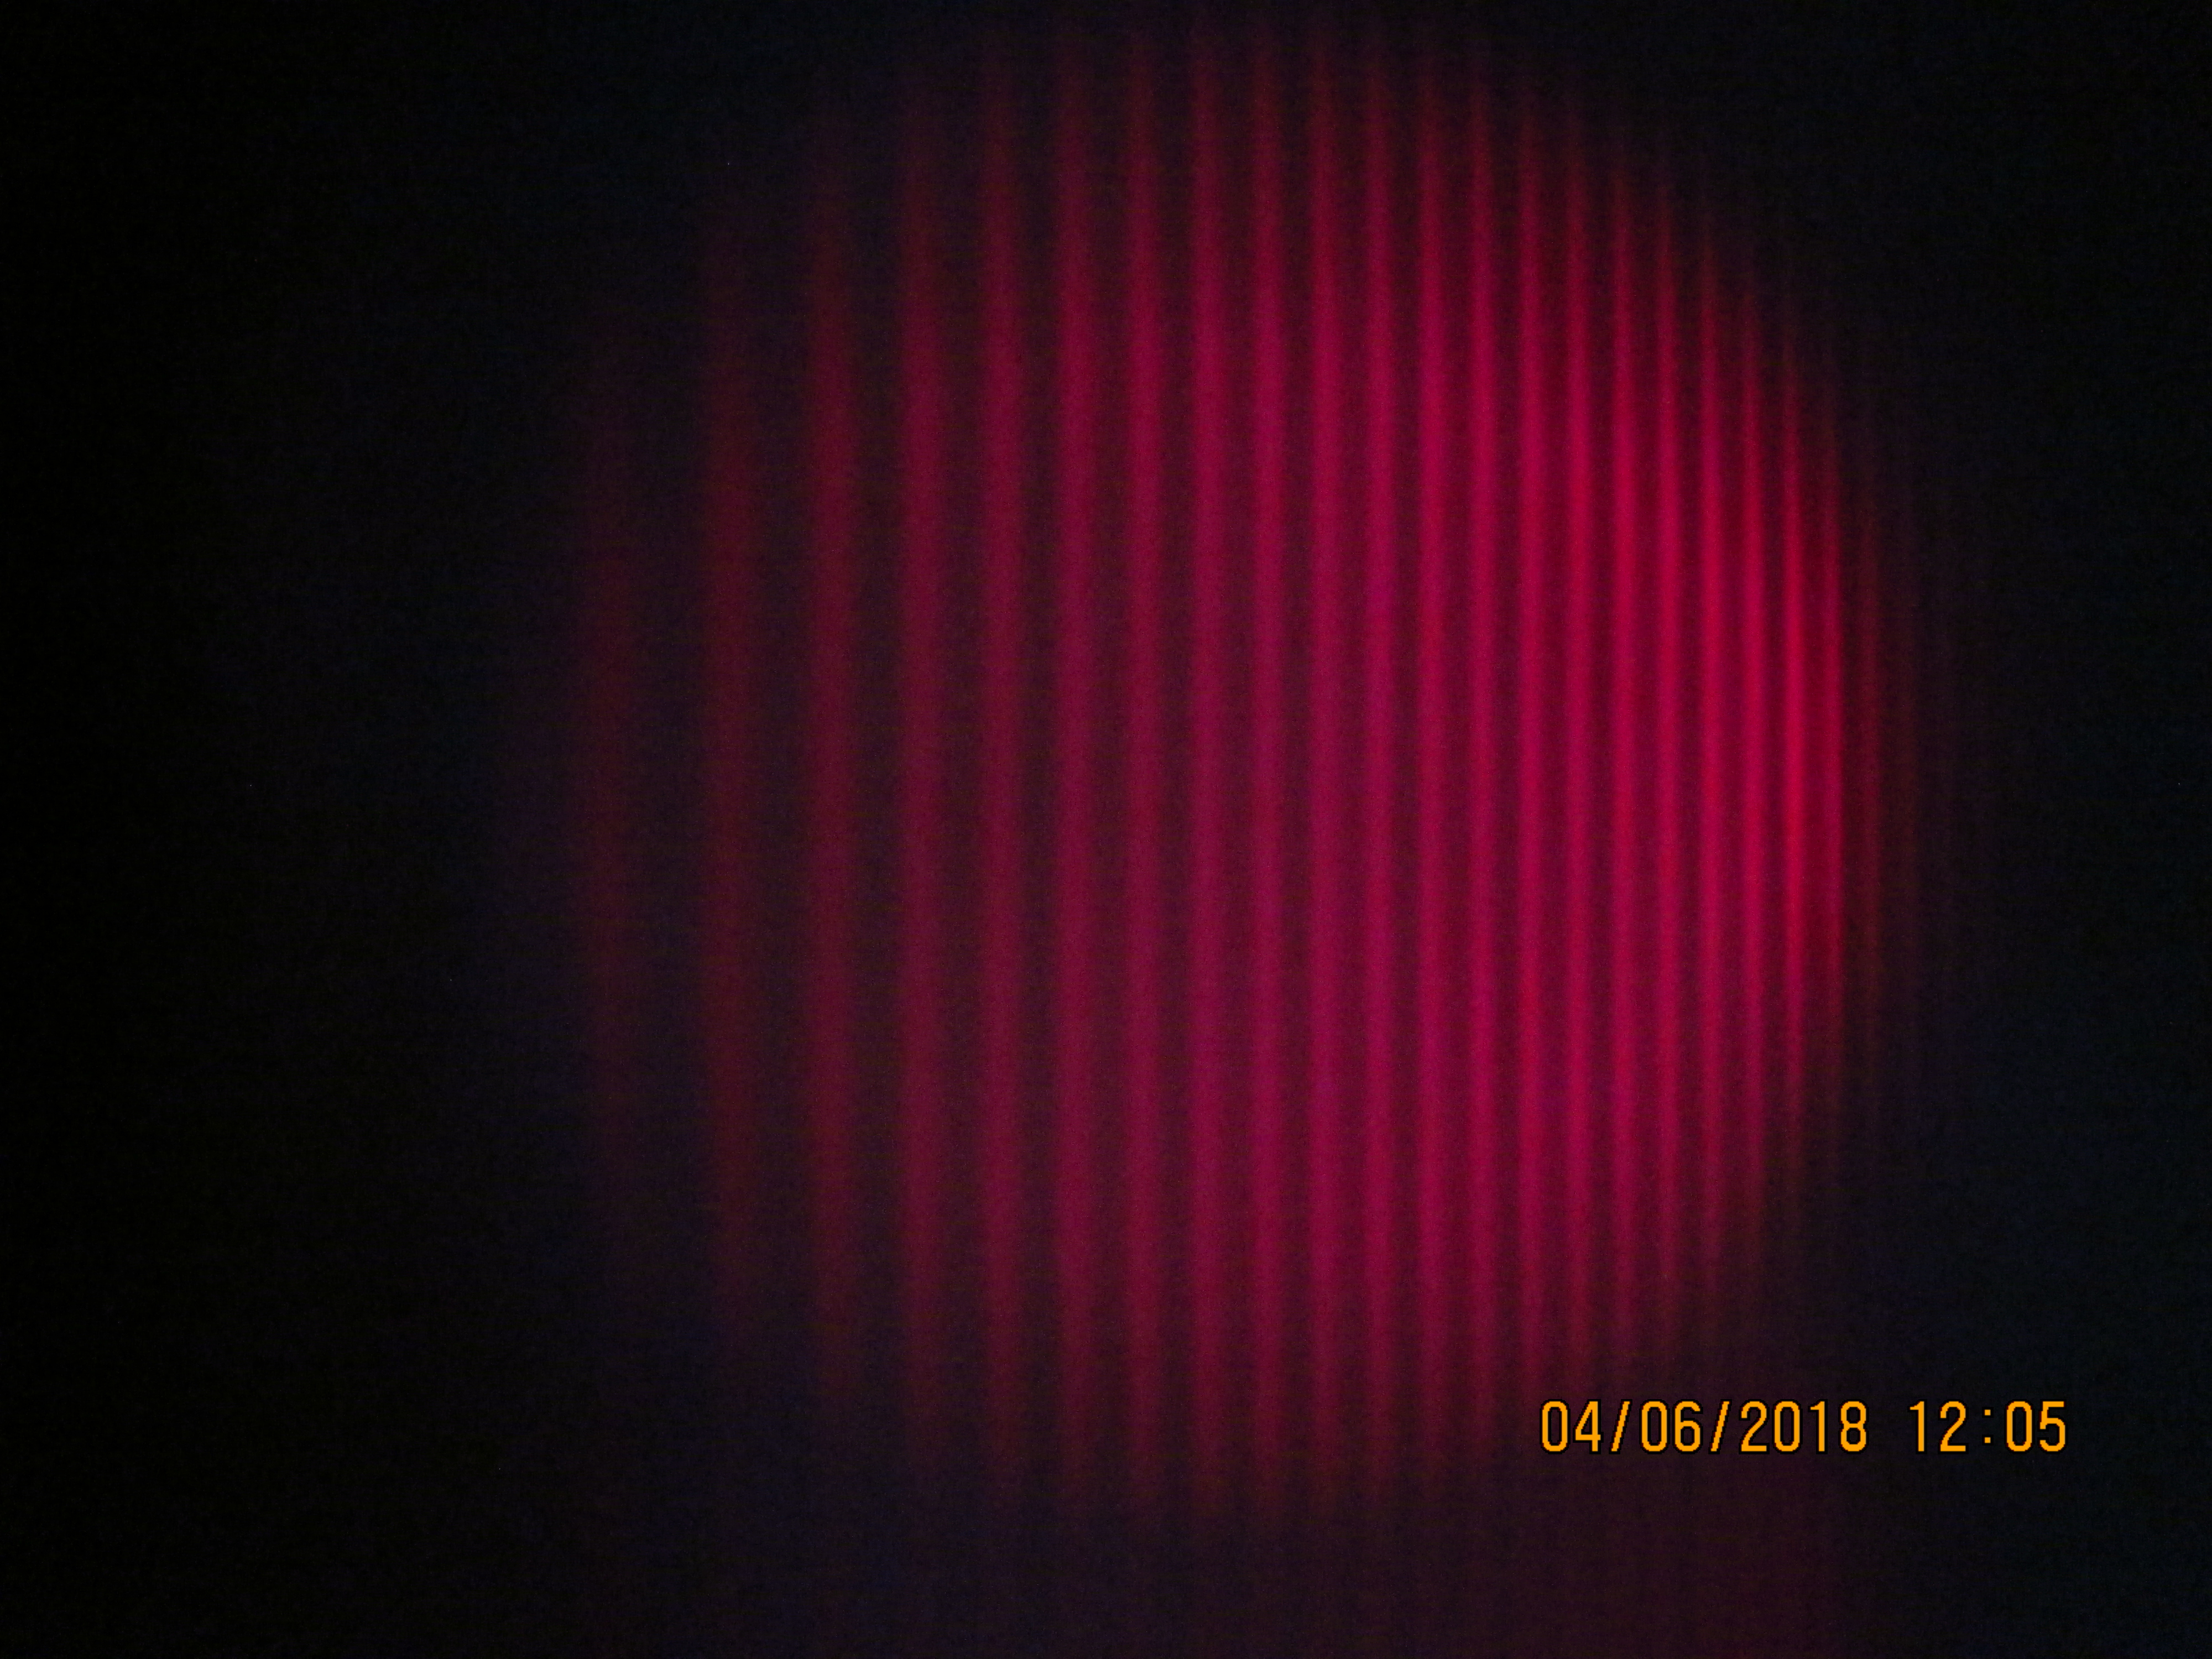
\includegraphics[width=0.95\textwidth]{graphics/auswertung/IMG_1632.png}
  \caption{rote $\sigma$-Linie mit Magnetfeld.}
  \label{}
\end{figure}

\begin{table}
  \centering
  \caption{rote $\sigma$-Linie.}
  \label{tab:r_sigma}
  \begin{tabular}{S[table-format=3] S[table-format=3] S[table-format=2.3] S[table-format=1.3] @{${}\pm{}$} S[table-format=1.3]}
    \toprule
    {$\upD s \:/\: $px} & {$\symup{\delta} s \:/\: $px} & {$\symup{\delta}\lambda \:/\: $pm} & \multicolumn{2}{c}{Landé-Faktor $g$} \\
    \midrule
    367 & 192 & 12.794 & 1.108 & 0.010 \\
    304 & 150 & 12.067 & 1.045 & 0.010 \\
    261 & 126 & 11.806 & 1.022 & 0.010 \\
    236 & 106 & 10.984 & 0.951 & 0.009 \\
    213 &  94 & 10.792 & 0.934 & 0.009 \\
    199 &  90 & 11.060 & 0.958 & 0.009 \\
    190 &  84 & 10.812 & 0.936 & 0.009 \\
    177 &  76 & 10.500 & 0.909 & 0.009 \\
    167 &  76 & 11.129 & 0.964 & 0.009 \\
    \bottomrule
  \end{tabular}
\end{table}

rot sigma: $\num{0.981 \pm  0.009}$
Magnetfeld: $\SI{597 \pm 6}{mT}$

\begin{figure}
  \centering
  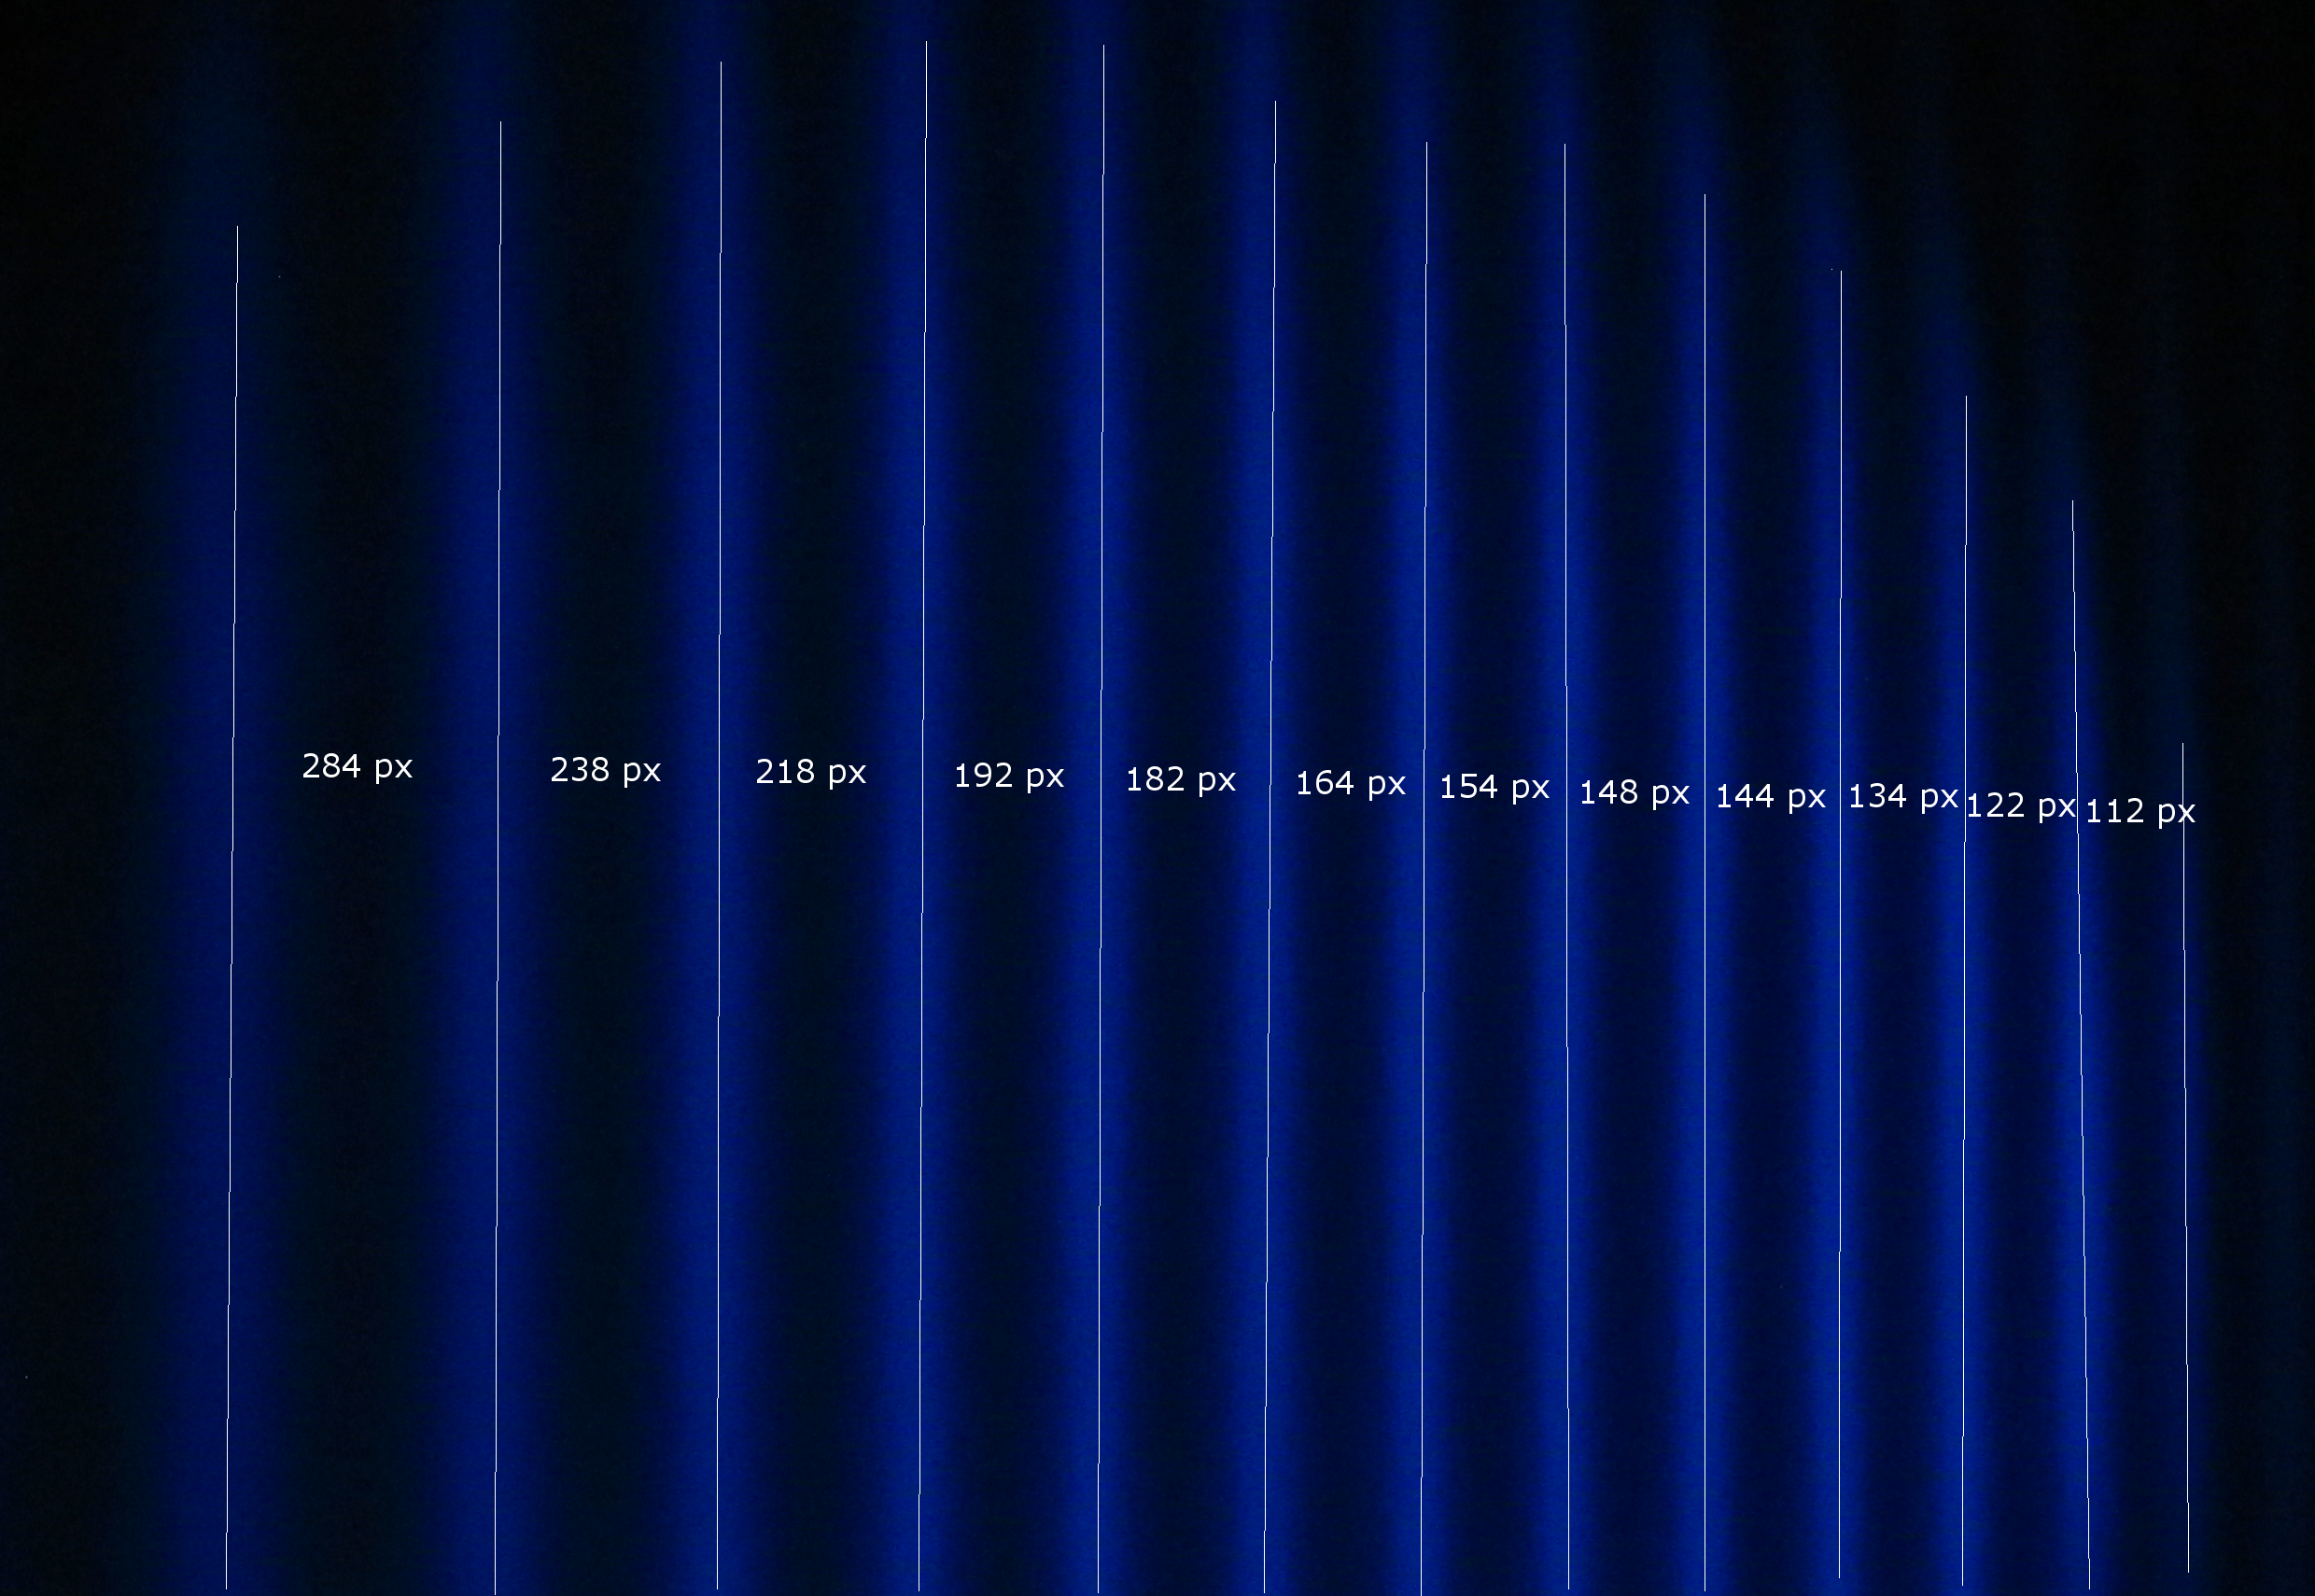
\includegraphics[width=0.95\textwidth]{graphics/auswertung/IMG_1635.png}
  \caption{blaue $\pi$-Linie ohne Magnetfeld.}
  \label{}
\end{figure}
\begin{figure}
  \centering
  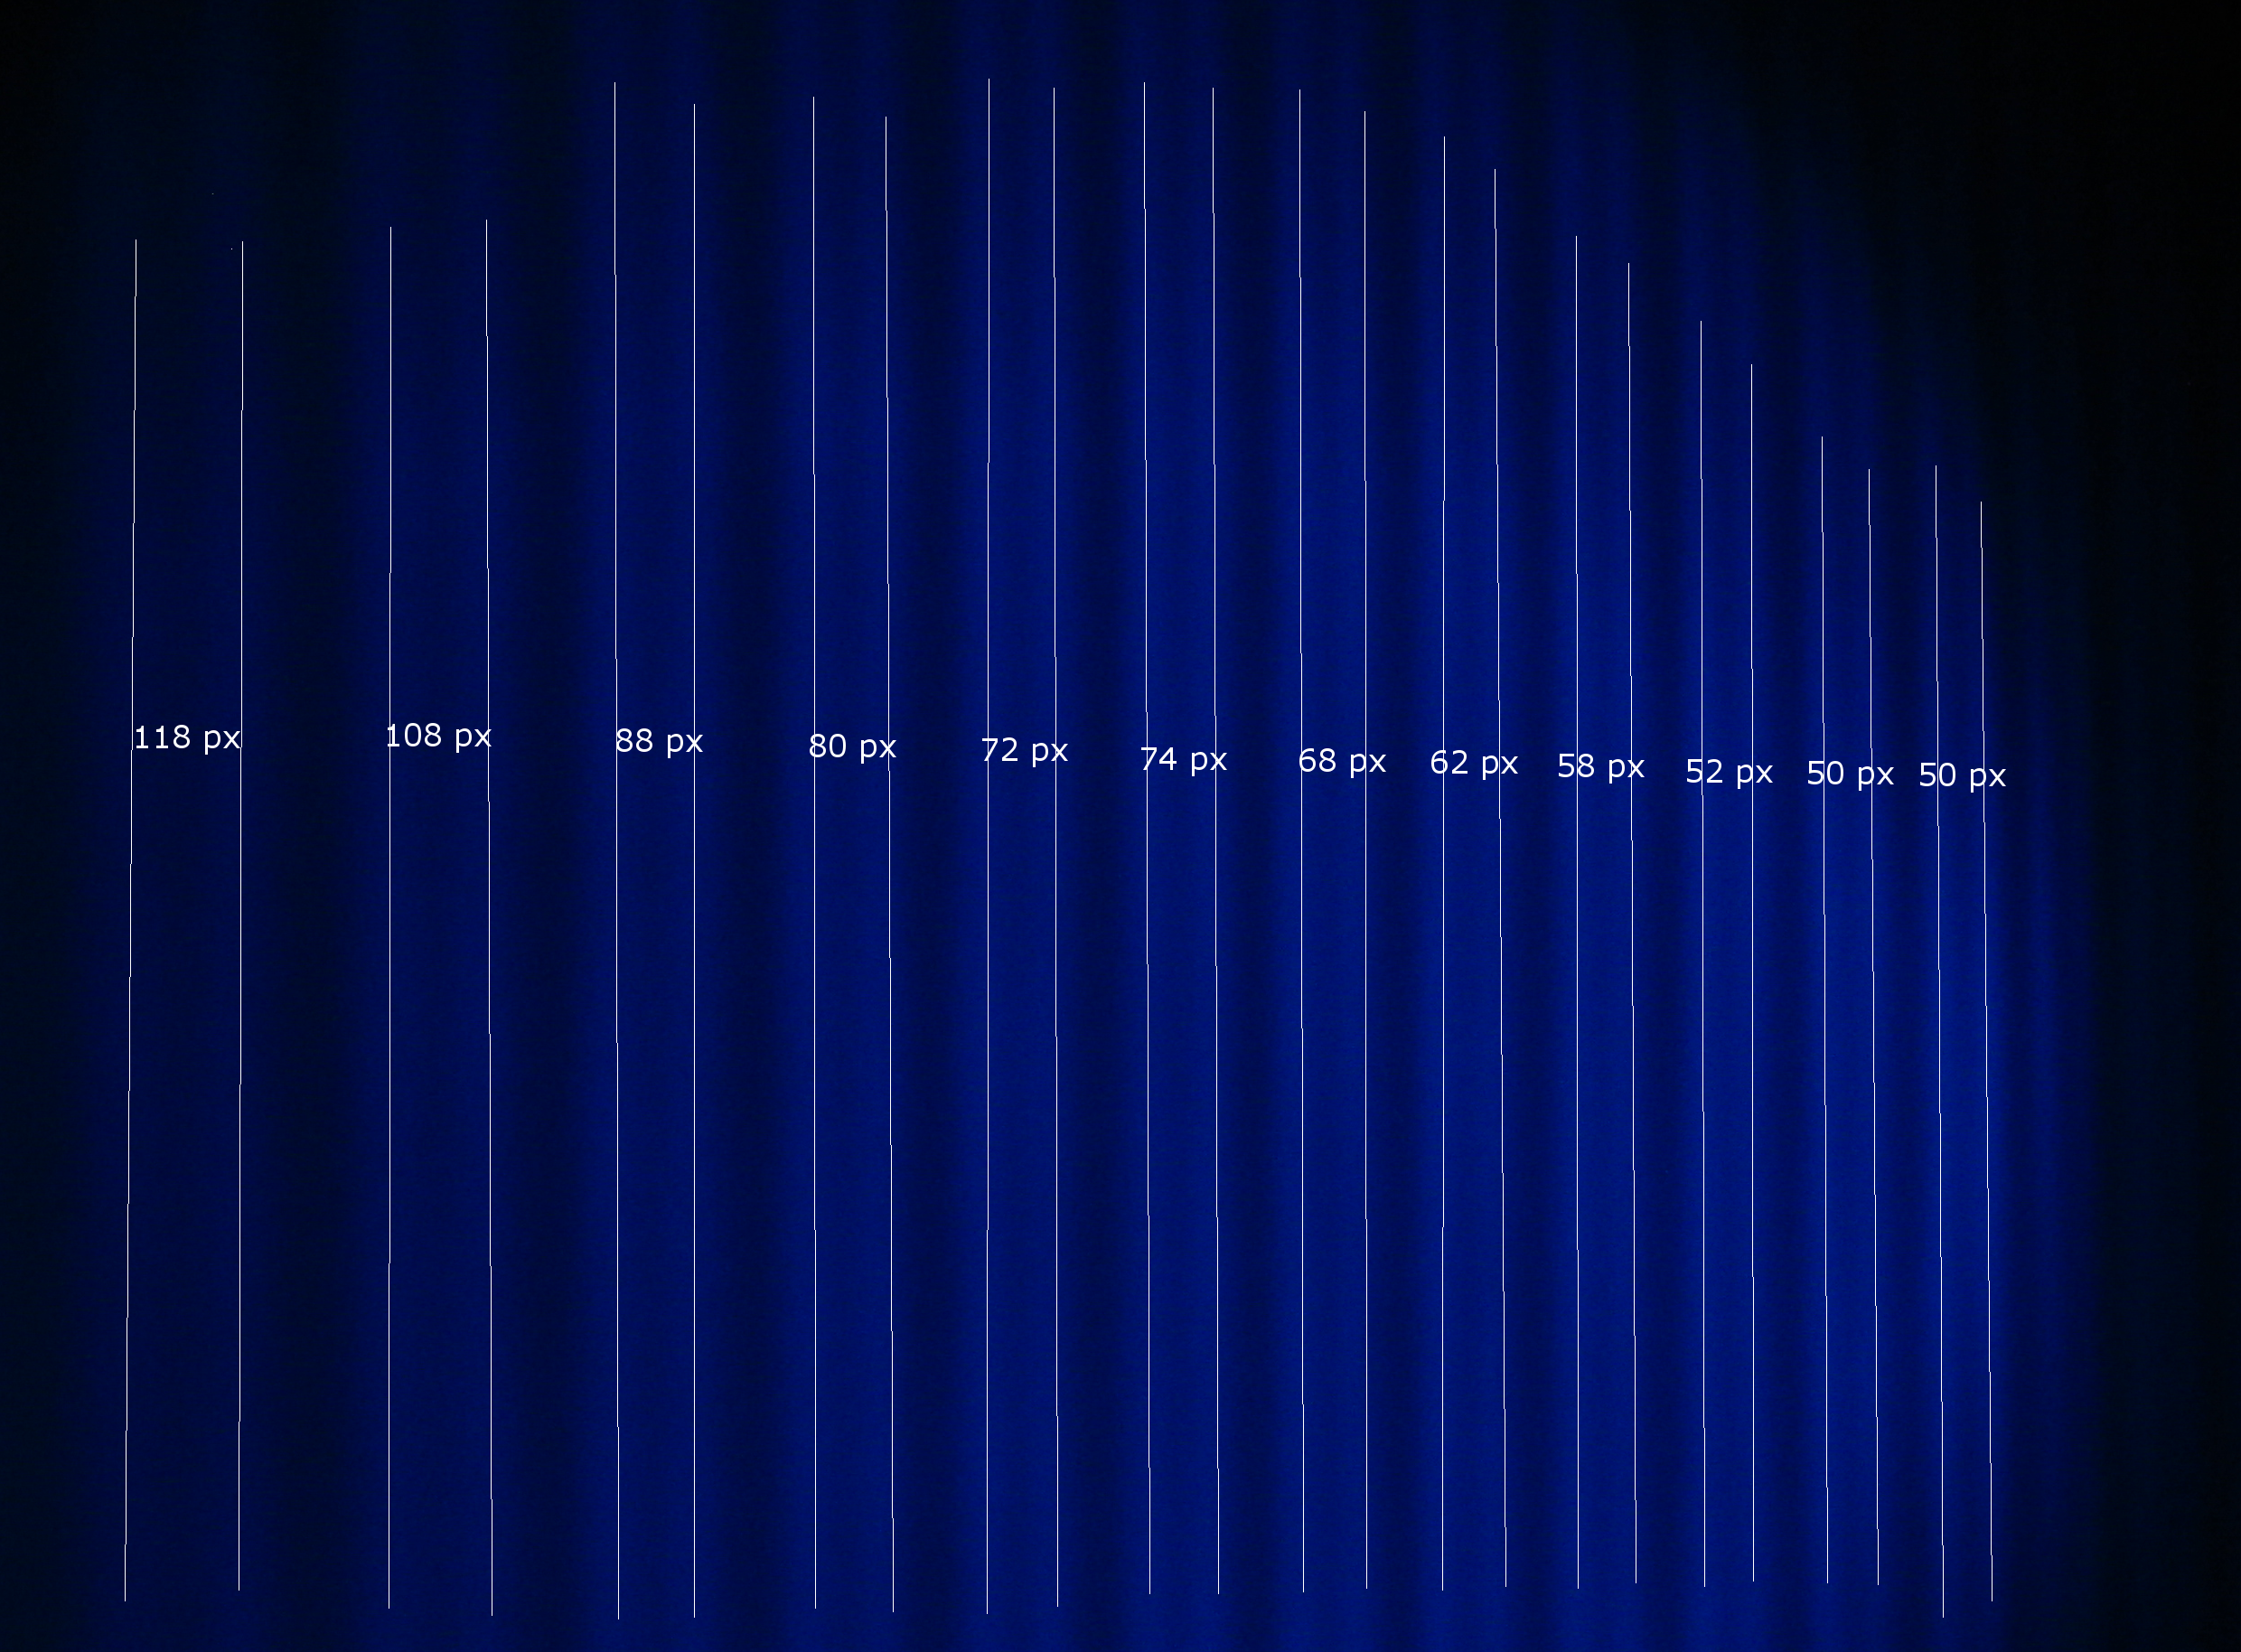
\includegraphics[width=0.95\textwidth]{graphics/auswertung/IMG_1644.png}
  \caption{blaue $\pi$-Linie mit Magnetfeld.}
  \label{}
\end{figure}

\begin{table}
  \centering
  \caption{blaue $\pi$-Linie.}
  \label{tab:r_sigma}
  \begin{tabular}{S[table-format=3] S[table-format=3] S[table-format=2.3] S[table-format=1.3] @{${}\pm{}$} S[table-format=1.3]}
    \toprule
    {$\upD s \:/\: $px} & {$\symup{\delta} s \:/\: $px} & {$\symup{\delta}\lambda \:/\: $pm} & \multicolumn{2}{c}{Landé-Faktor $g$} \\
    \midrule
    284 & 118 & 5.599 & 0.519 & 0.004 \\
    238 & 108 & 6.115 & 0.567 & 0.004 \\
    218 &  88 & 5.439 & 0.505 & 0.004 \\
    192 &  80 & 5.615 & 0.521 & 0.004 \\
    182 &  72 & 5.331 & 0.495 & 0.004 \\
    164 &  74 & 6.080 & 0.564 & 0.004 \\
    154 &  68 & 5.950 & 0.552 & 0.004 \\
    148 &  62 & 5.645 & 0.524 & 0.004 \\
    144 &  58 & 5.427 & 0.503 & 0.004 \\
    134 &  52 & 5.229 & 0.485 & 0.004 \\
    122 &  50 & 5.523 & 0.512 & 0.004 \\
    112 &  50 & 6.016 & 0.558 & 0.004 \\
    \bottomrule
  \end{tabular}
\end{table}

blau pi: $\num{0.525 \pm 0.004}$
Magnetfeld: $\SI{1002 \pm 8}{mT}$

\begin{figure}
  \centering
  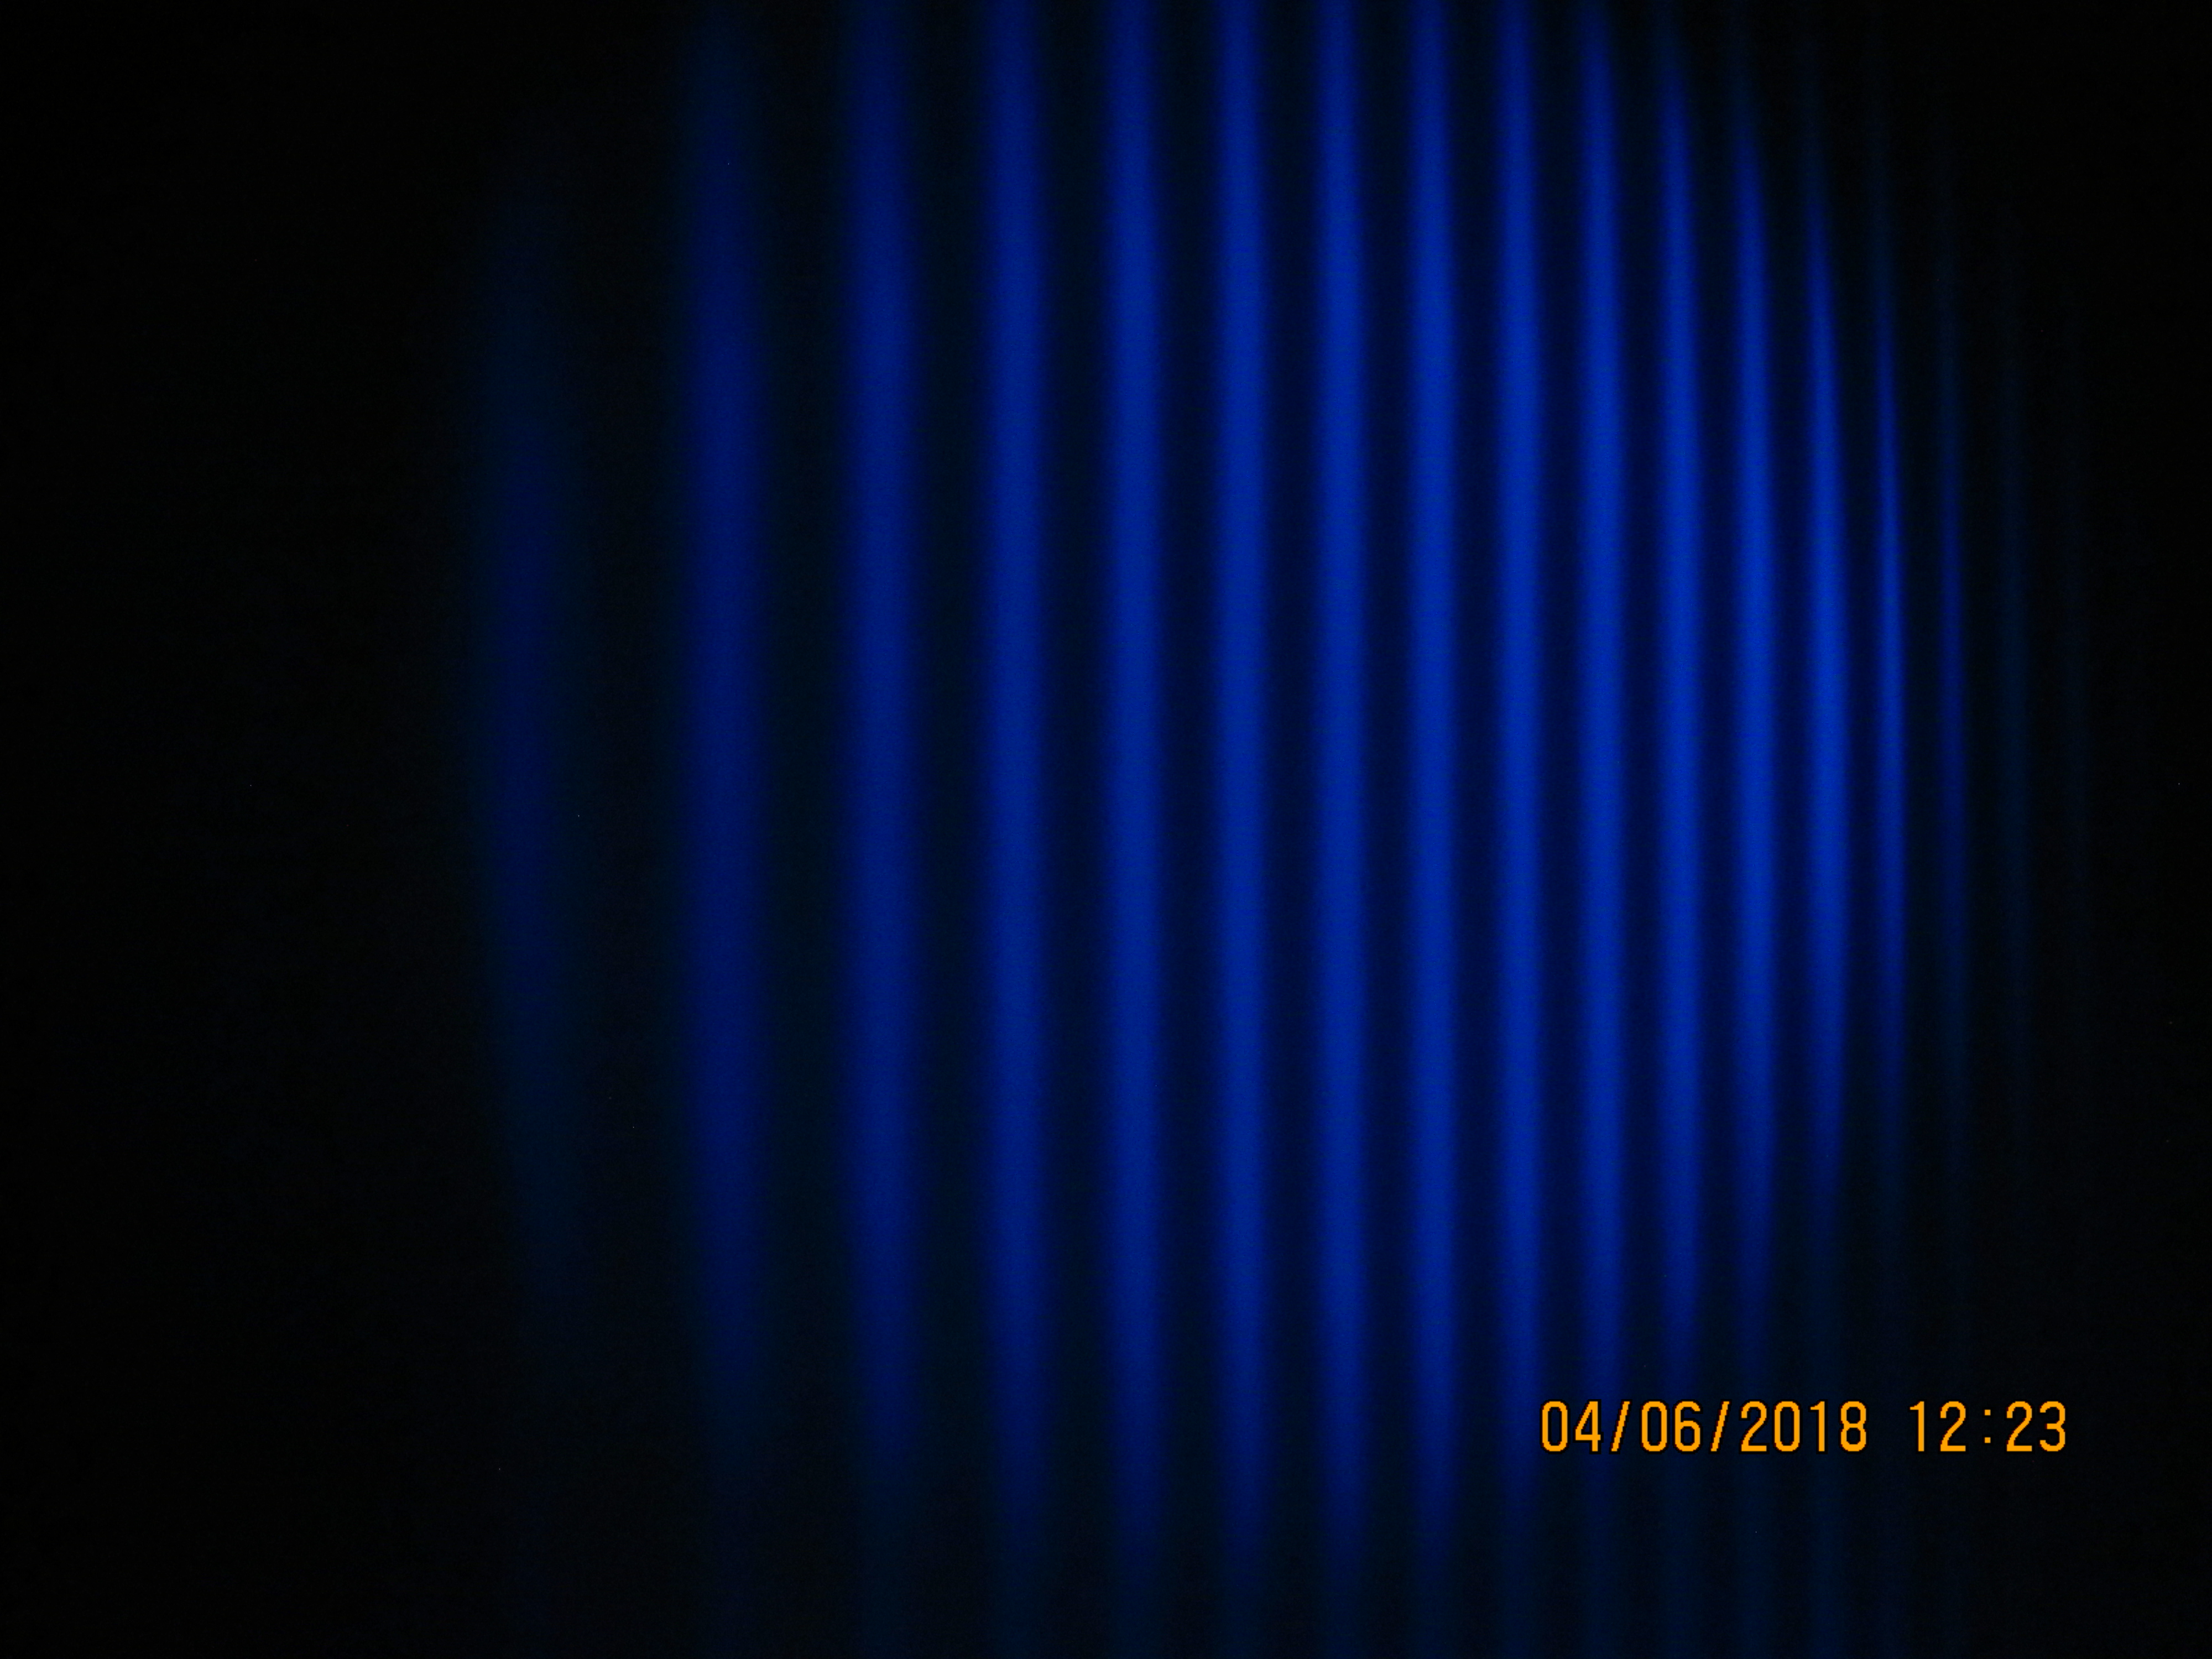
\includegraphics[width=0.95\textwidth]{graphics/auswertung/IMG_1637.png}
  \caption{blaue $\sigma$-Linie ohne Magnetfeld.}
  \label{}
\end{figure}
\begin{figure}
  \centering
  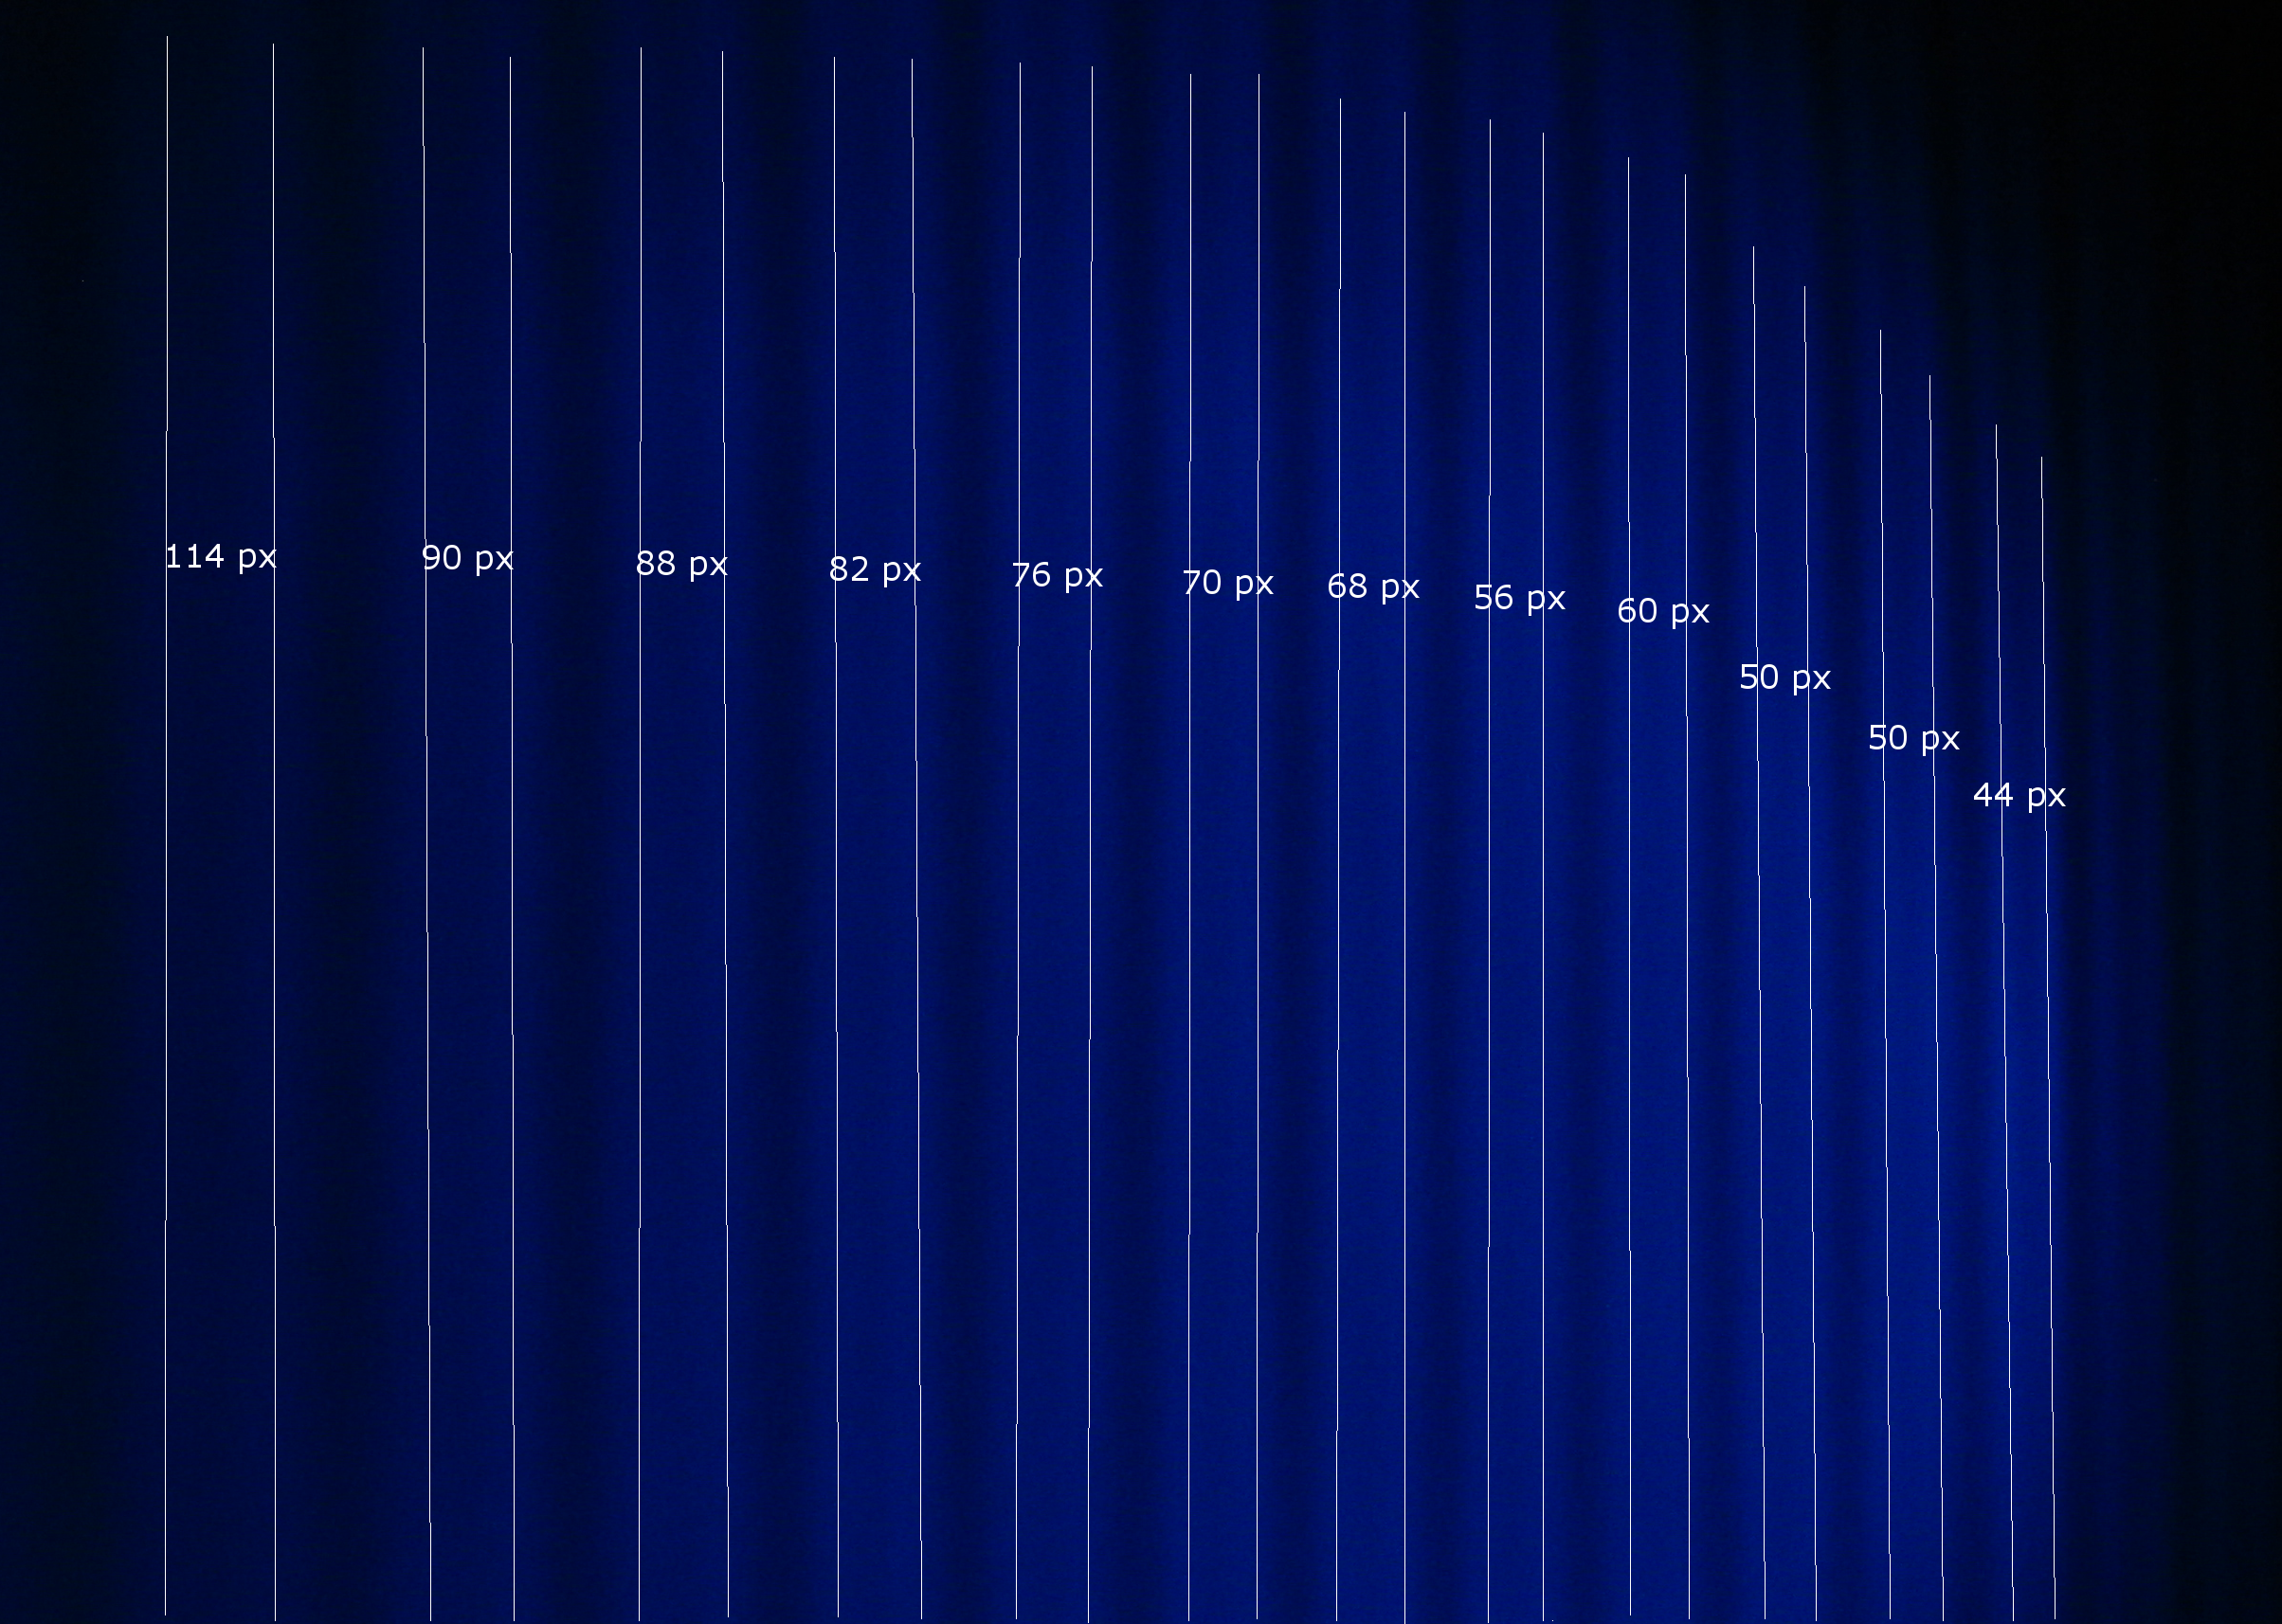
\includegraphics[width=0.95\textwidth]{graphics/auswertung/IMG_1641.png}
  \caption{blaue $\sigma$-Linie mit Magnetfeld.}
  \label{}
\end{figure}

\begin{table}
  \centering
  \caption{blaue $\sigma$-Linie.}
  \label{tab:r_sigma}
  \begin{tabular}{S[table-format=3] S[table-format=3] S[table-format=2.3] S[table-format=1.3] @{${}\pm{}$} S[table-format=1.3]}
    \toprule
    {$\upD s \:/\: $px} & {$\symup{\delta} s \:/\: $px} & {$\symup{\delta}\lambda \:/\: $pm} & \multicolumn{2}{c}{Landé-Faktor $g$} \\
    \midrule
    282 & 114 & 5.447 & 1.387 & 0.018 \\
    248 &  90 & 4.890 & 1.245 & 0.016 \\
    208 &  88 & 5.701 & 1.451 & 0.018 \\
    196 &  82 & 5.638 & 1.435 & 0.018 \\
    180 &  76 & 5.689 & 1.448 & 0.018 \\
    162 &  70 & 5.823 & 1.482 & 0.019 \\
    156 &  68 & 5.874 & 1.495 & 0.019 \\
    146 &  56 & 5.168 & 1.316 & 0.017 \\
    140 &  60 & 5.775 & 1.470 & 0.019 \\
    130 &  50 & 5.183 & 1.319 & 0.017 \\
    132 &  50 & 5.104 & 1.299 & 0.017 \\
    110 &  44 & 5.390 & 1.372 & 0.017 \\
    \bottomrule
  \end{tabular}
\end{table}

blau sigma: $\num{1.39  \pm  0.02}$
Magnetfeld: $\SI{365 \pm 5}{mT}$
